\subsection{Propulsion (PRP)}

The propulsion subsystem is responsible for changing the spacecraft's orbit. In the first phase of the cubesat lifetime, propulsion is necessary for proper satellite positioning as well as minor orbit corrections and collision avoidance during the remainder of its lifetime. To position the satellites, their time-position must be  adjusted. The aim is to create a constellation of satellites to provide complete communications coverage over the Earth's surface. The proposed constellation shall be composed of 8 polar orbiting families of satellites. Each family shall be comprised of 9 cubesats.

Changing the time-position of one satellite along the orbit is known as \textbf{orbit phasing}. As shown in Figure \ref{fig:orbit_phasing} the satellite can be given an increase in velocity to lower the orbital altitude, thus decreasing the orbital period. When the satellite completes the phasing orbit, another velocity change is required to return the satellite to the desired orbit.

\begin{figure}[h!]
	\centering
	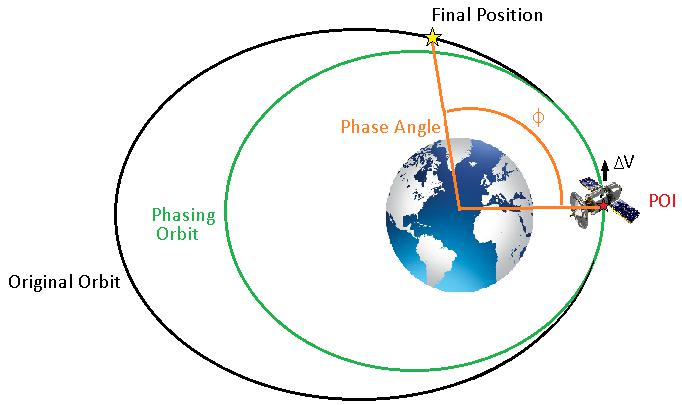
\includegraphics[scale=0.5]{img/Orbit_Phase.jpg}
	\caption{Orbit Phasing}
	\label{fig:orbit_phasing}
\end{figure}

There are a number of methods of achieving the desired orbits for this constellation.
\begin{enumerate}
	\item Differing $\Delta V$
	In this scenario, nine satellites are launched into polar orbit at an altitude of 625km, the desired orbit. Each satellite then does one phasing orbit, using differing $\Delta V$ and returns to it's polar orbit. This method is the fastest but requires different amounts of propellant for each satellite.
	\item Differing number of phasing orbits.
	Here, the satellites are launched to the same orbit as in the previous case. However, each satellite, except one, experiences the same $\Delta V$ but they complete a different number of phasing orbits before returning to their original orbit. If we number the satellites as n=1:9, then satellite n will complete n-1 phasing orbits. This method is slower than the first method but it involves significantly less propellant as n increases.
	\item Launch to phasing orbit
	The third method is to launch all nine satellites to the 'phasing orbit'. As with method 2, the satellites would complete n-1 phasing orbits before using a velocity kick to reach the desired orbit. The benefit of this method is that eight of the satellites would only need one velocity change, rather than two, however, satellite 1 in the orbital family would need one extra velocity kick. Clearly, method 3 uses the least amount of propellant of all three methods, while also having the benefit of standardising the satellites' propulsion systems as each one would require an equal amount of propellant.
\end{enumerate}

\subsubsection{Required $\Delta V$}
For an orbit of nine satellites, $\phi = 40^{\circ}$. To calculate the required $\Delta V$ the following equations can be used, where subscript 1 refers to the original orbit and subscript 2 refers to the final orbit.

\begin{equation}
	E=2tan^{-1}\bigg(\sqrt{\frac{1-e_1}{1+e_1}tan\frac{\phi}{2}} \bigg)
	\label{MMeq1}
\end{equation}

\begin{equation}
	t=\frac{T_1}{2\pi}(E - e_1 sinE)
	\label{MMeq2}
\end{equation}

The required time period of the final orbit is then given by using equation \ref{MMeq3}.

\begin{equation}
	T_2 = T_1 -t
	\label{MMeq3}
\end{equation}

The final orbit semimajor axis can then be determined by using equation \ref{MMeq4}.

\begin{equation}
	a_2 = \bigg(\frac{\sqrt{\mu}T_2}{2\pi}\bigg)^{\frac{2}{3}}
	\label{MMeq4}
\end{equation}

The angular momentum of the orbit can then be calculated by using equation \ref{MMeq5}.

\begin{equation}
	h_2 = \sqrt{2\mu}\sqrt{\frac{r_ar_p}{r_a+r_p}}
	\label{MMeq5}
\end{equation}

Finally, equation \ref{MMeq6} can be used to calculate the change in velocity, $\Delta V$ at the Point of Impulse.

\begin{equation}
	\Delta V = v_2 - v_1 = \frac{h_2}{r}-\frac{h_1}{r}
	\label{MMeq6}
\end{equation}

The result of these calculations shows that a $\Delta V$ of $350 m/s$ is needed to transfer from the phasing orbit to the circular constellation orbit.

With the required $\Delta V$ known, the Tsiolkovsky rocket equation (equation \ref{MMeq7}) can be derived to estimate the required mass fraction of propellant for various propulsion systems (equation \ref{MMeq8}). To do this, the effective exhaust velocity of the thruster must be known.

\begin{equation}
	\Delta V = v_e ln \frac{m_0}{m_f}
	\label{MMeq7}
\end{equation}

\begin{equation}
	\frac{m_p}{m_0} = 1-exp\bigg(-\frac{\Delta V}{v_e}\bigg)
	\label{MMeq8}
\end{equation}

As $v_e = g_0 I_{sp}$ we can approximate the mass fractions of propellant needed for a variety of thrusters of given $I_{sp}$, by Tummala and Dutta in \cite{Tummala}. From the previous equations, it is clear that a high $I_{sp}$ is desirable to minimise the mass fraction of the propellant, and thereby the mass of the propulsion system. Here, the propulsion system with the greatest Specific Impulse of each propellant type, except solar sails, is examined.

\begin{table}[h!]
	\centering
	\begin{tabular}{c c c c c c }
		\hline
		Propellant & Manufacturer & Engine & $I_{sp}$ & $v_e$ & $m_p/m_0$ \\
		\hline
		Cold Gas & GOMSpace & MEMS Cold Gas & 62 & 608.22 & 0.438 \\
		Liquid & Tethers Unlimited & HYDROS & 256 & 2511.36 & 0.130 \\
		Solid & Orbital ATK & STAR 4G & 269.4 & 2642.814 & 0.124 \\
		Resistojet & Busek & AMR & 150 & 1471.5 & 0.212 \\
		Radio Frequency Ion & Busek & BIT-3 & 2500 & 24525 & 0.014 \\
		Hall Effect & Sitael Aerospace & HT 400 & 1750 & 17167.5 & 0.020 \\
		Electrospray & Busek & BET-100 & 1800 & 17658 & 0.019 \\
		Arc Thrusters & Busek & MPACS & 830 & 8142.3 & 0.042 \\
		\hline
	\end{tabular}
	\caption{$I_{sp}$ and $v_e$ for various cubesat propulsion systems with corresponding mass fraction of propellant needed to obtain $\Delta V$ of $350 m/s$}
	\label{MMtab1}
\end{table}

Proceeding with the four engines which require less than 5\% propellant mass, the practical limitations of the engines are laid out in table \ref{MMtab2}.
\\
\begin{table}[h!]
	\centering
	\begin{tabular}{c c c c c }
		\hline
		Propellant & Manufacturer & Engine & Thruster Mass(kg) & Power(W) \\
		\hline
		Radio Frequency Ion & Busek & BIT-3 & 0.2 & 20-70 \\
		Hall Effect & Sitael Aerospace & HT 400 & 0.9 & 250-800 \\
		Electrospray & Busek & BET-100 & 0.329 & 5.5 \\
		Arc Thrusters & Busek & MPACS & 0.5 & 7.5 \\
		\hline
	\end{tabular}
	\caption{$I_{sp}$ and $v_e$ for cubesat propulsion systems with corresponding thruster unit mass and nominal power consumption}
	\label{MMtab2}
\end{table}
\\
The power requirements of the Busek BIT-3 engine are unrealistic for a cubesat, therefore the best engine for this application is the Busek BET-100 due to the very low mass fraction of propellant required and the low power and weight associated with the engine. The module is 9 cm x 9 cm x 4 cm in size and delivers 100$\mu N$ of thrust at Specific Impulse of 1800 - 2300 s. A single module can deliver 85m/s to a 4kg satellite, thus the proposed propulsion system incorporates engines in parallel, the quantity depending on the final wet mass of the satellite, including the mass of the propulsion system itself.
